\documentclass[11pt,twoside,a4paper]{report}

% Intra-PDF Links and Bookmarks 
\usepackage[colorlinks=true,linkcolor=black,urlcolor=blue,bookmarksopen=true]{hyperref}
\usepackage[open,openlevel=1]{bookmark}

% A4, 1.91cm margins, header+footer
\usepackage[a4paper, margin=1.91cm, top=2.91cm, bottom=2.91cm]{geometry}
\usepackage{fancyhdr}
\pagestyle{fancy}
\fancyhf{}
\setlength{\headheight}{15.2pt}
\fancyfoot[LE,RO]{ \thepage }
\fancyfoot[RE,LO]{ \textit{Timothy Langer 2021} }

% Use UTF-8 so that we can have lots of nice characters!
\usepackage[utf8]{inputenc}
\usepackage[british]{babel}

% Maths symbols and packages
\usepackage{amsmath}
\usepackage{amssymb}
\usepackage{gensymb}

% easy way to include SI units in text
\usepackage{siunitx}

% Apply spacing in between paragraphs
\setlength{\parskip}{1em}
\setlength{\parindent}{0pt}

% Add diagrams and images support
\usepackage{graphicx}
\graphicspath{ {./images/} }
\usepackage{caption}

% Mathematics typesetting support 
\usepackage{commath}

% Multiple columns
\usepackage{multicol}

% bibliography
\usepackage{csquotes}
\usepackage[
backend=biber,
style=numeric,
sorting=ynt,
urldate=long,
]{biblatex}

\addbibresource{./citations.bib}

%\usepackage[superscript,biblabel]{cite}

% better chapter titles
\usepackage[T1]{fontenc}
\usepackage{titlesec, blindtext, color}

% shorthands for custom chapter format
\definecolor{gray75}{gray}{0.75}
\newcommand{\hsp}{\hspace{20pt}}

% more compact chapter titles
\titleformat{\chapter}{\Huge\bfseries}{\thechapter\hsp\textcolor{gray75}{|}\hsp}{0pt}{\Huge\bfseries}
% less top/bottom padding around chapter titles
\titlespacing{\chapter}{0pt}{*0}{*1}

\pdfsuppresswarningpagegroup=1

\author{Timothy Langer}
\title{Smartphone-based tracking of rowing training}
\date{\today}

% this defines the \@title, \@author and \@date commands
\makeatletter

\fancyhead[LE,RO]{ \@title }

\begin{document}

\begin{titlepage}
  \centering
  \vspace*{1cm}
  {\bfseries \huge \@title \par}
  \vspace{2cm}
  {\large AQA Computer Science A-Level \par Non-Examined Assessment \par}
  \vspace{1.5cm}
  {\LARGE \@author \par}
  \vfill
  
\includegraphics[width=0.2\textwidth]{sps-logo} \par
  {\scshape\LARGE St Paul's School \par}
  Dr~C.~A.~Harrison \par
  \vspace{1cm}
  {\large \@date \par}
  \vspace*{1cm}
\end{titlepage}

% end the titling area
\makeatother

\tableofcontents

\chapter{Analysis}

\section{Introduction to rowing}

Rowing in its modern form developed in England in the $1700$s, with the first recorded race held in $1715$. 
Nowadays, it is particularly popular in the UK and US. 
The Boat Race on television has over seven million viewers, with a further $250,000$ attending in person.\cite{the_boat_race} 

Two kinds of competitions exist: head races and regattas. 
A head race is one where competitors compete for the fastest time take to row a given distance. 
The outcome of the race is not clear until the race is over and times for every boat have been compiled.
A regatta involves side-by-side racing, across several lanes, usually over a course of $2000 \si{\meter}$.
Regattas are preferable for spectating, because it is obvious as to which boat is physically in the lead.
Typically, head races take place in in the autumn and winter, whereas regattas are frequent in late spring and summer.
Head races in particular require accurate timing and tracking of competitors' boats, seeing as the results are based on this information.

\subsection{The rowing stroke}

\begin{figure}[ht]
    \centering
    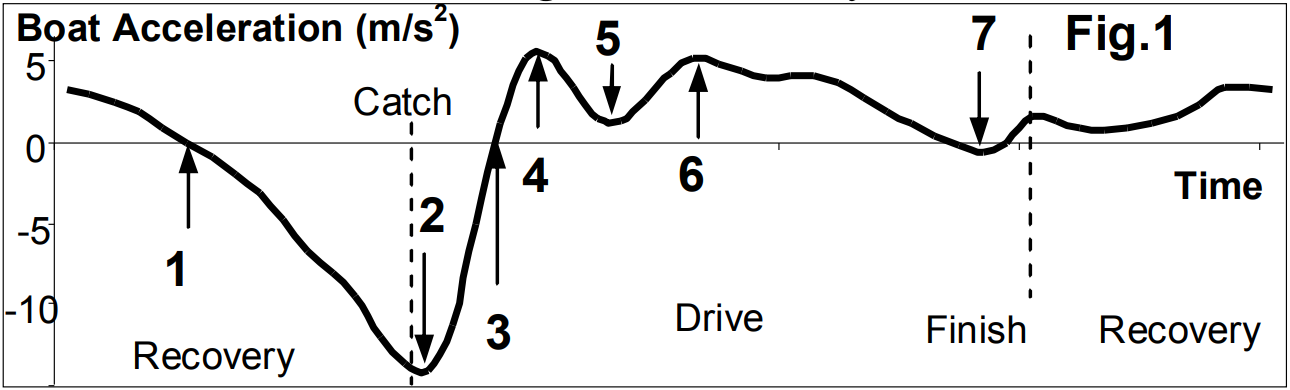
\includegraphics[width=0.7\textwidth]{rowing-stroke}
    \caption{Typical pattern of boat acceleration during the stroke cycle \cite{dr_valery_kleshnev_analysis_2012}}
    \label{fig:rowing-stroke}
\end{figure}

Rowing (and/or sculling) involves the propulsion of a racing shell \footnote{the long, light and narrow boat used for rowing} through the water, using either one or two oars. 
Rowing is cyclic and repetitive in its nature; every stroke is alike. 
The rowing stroke consists of two phases: the \textit{drive} and the \textit{recovery}. 
During the drive, the athelete pushes with their legs, moving towards the bow of the boat, with the oars in the water, thus accelerating the boat.
In the recovery, the athlete slides to the rear of the boat, while the boat slightly decelerates.
Figure \ref{fig:rowing-stroke} shows a typical acceleration pattern of a single stroke.

Given the fact that this acceleration pattern repeats with little fluctuation, it should not be difficult to isolate when a the pattern repeats, and thus calculate the number of strokes being taken per minute. By combining this data with GPS readings, one can also calculate the distance the boat travels per stroke.

\subsection{Practical considerations}

Although increasingly common, not many smartphones have a sufficient ingress protection rating to be comfortably taken into the boat. 
It is necessary to consider the requirement of a waterproof case, clamp or other holder that would allow the device to be affixed securely to the boat and prevent water damage in case of rain, waves or capsizing. 
One example would be a waterproof jogging armband: these are inexpensive, can be wrapped around a wing rigger \footnote{modern version of an \href{https://en.wikipedia.org/wiki/Outrigger}{outrigger} that spans across the middle from one gunwhale to the other} and are a low barrier to entry.

\section{Existing solutions}

\subsection{Nielsen-Kellerman SpeedCoach}

The \href{https://nksports.com/speedcoach-gps-2}{NK SpeedCoach \rightsreserved GPS (Model 2)} is a popular performance monitor for rowing on the water. 
It displays realtime information including split, stroke rate and the time and distance rowed. 
The first model used a physical magnet installed in the boat to record stroke rate, however, the second edition uses an inbuilt accelerometer for this and is completely wireless. 

An optional \textit{Training Pack} is available with Model 2 that adds software features such as Bluetooth support for heart rate monitor and synchronising training data to a smartphone.

The basic edition of the second model retails for \textsterling $399$; the \textit{Training Pack} is another \textsterling $99$.

\section{Specification}

The program \textbf{must}:
\begin{enumerate}
  \item collect data during a rowing session using nothing but the hardware on the smartphone,
  \item require minimal interaction from the athlete, and ideally none at all,
  \item output a \href{https://developer.garmin.com/fit/file-types/activity/}{\texttt{FIT} activity file} at the end of the session that can be imported into 3rd-party software, such as \href{https://strava.com}{Strava}, containing
  \begin{itemize}
    \item the geolocation of the boat,
    \item the speed of the boat,
    \item the cadence, or stroke rate, of the rowers,
    \item the heart rate, if connected, from any supported heart rate monitor.
  \end{itemize}
\end{enumerate}

The program \textbf{may}:
\begin{enumerate}
  \item display a user interface with realtime stroke rate, speed, and heart rate,
  \item calculate additional metrics about the stroke, such as
    \begin{itemize}
      \item the ratio of time spent on the drive to time spent on the recovery,
      \item how much check \footnote{rapid, jolting change in the acceleration of the boat} there is at the catch,
      \item how balanced the boat is during the session,
    \end{itemize}
  \item provide automated synchronisation of training sessions to a 3rd-party activity tracking website, such as Strava, 
\end{enumerate}

\chapter{Design}

\section{Input}

\subsection{Device sensors}

Almost all handheld Android smartphones have an accelerometer, since this is necessary for the screen auto-rotation feature, and many also feature either a gyroscope or a magnetometer. \cite{android_motion_sensors} 
The key component for this project is the accelerometer, however, the gyroscope and magnetometer could be used to improve the accuracy of the data.

As part of the Android software stack, a virtual sensor is also available that filters out acceleration due to gravity from the signal. \cite{android_linear_accel} 

It would be sensible to sample all the available motions sensors, both virtual and physical, and record all the raw values. 
By storing the raw data, it can be more thoroughly analysed once the training session is over and battery drain is not of concern.

\section{Processing data}

\subsection{Basic method}

The acceleration and linear acceleration sensors output a vector with $x$, $y$ and $z$ axes, which are oriented relative to the device, with the $z$-axis coming out of the screen of the device. 
Since the boat is travelling linearly and we do not need an accurate numeric value for the accleration, it is enough to calculate the magnitude of the linear acceleration
\[
  \abs{\textbf{a}} = \sqrt{x^2 + y^2 + z^2} 
\] 
to obtain a repeating (with slight variation) pattern. By shape, one would expect a pattern similar to the absolute value of the acceleration pattern shown in in figure \ref{fig:rowing-stroke}.
Thus it would be reasonable to split the incoming signal at the instant when $\abs{\textbf{a}}$ peaks, that is, typically, at the catch. 
The number of strokes taken per minute is the reciprocal of the time taken for a single stroke.

\subsection{Device hardware}

The top $1822$ most popular Android devices on Geekbench, a popular benchmarking tool, have an average performance of $1018$, scoring slightly higher than a desktop Intel\textsuperscript{\textregistered} Core\texttrademark i$3$-$8100$ CPU. \cite{android_benchmarks} 

Given that this application should run on as many devices as possible, the core features must be optimised to perform well on lower-end devices.
Increased efficiency of the algorithms involved has the added benefit of reducing battery usage on higher-end devices too.

\medskip

\printbibliography[heading=bibintoc]

\end{document}
